\documentclass[12pt,fleqn,a4paper]{article}

\usepackage{latexsym}
\usepackage{url}
\usepackage{xspace}
\usepackage{epsfig}
\usepackage{psfrag}
\usepackage{a4wide}
\usepackage{marvosym}
\usepackage{amsmath,amsfonts,amssymb,amsthm,latexsym}
\usepackage{graphics,graphicx,color,subfigure}
\usepackage{fancyhdr}
\usepackage[english]{babel}
\usepackage[latin1]{inputenc}
\usepackage{algorithm}
\usepackage{algorithmic}
\documentclass{article}


\textheight 680pt
\textwidth 460pt
\topmargin -40pt
\oddsidemargin 5pt
\evensidemargin 5pt
\parindent 0pt

\pagestyle{fancyplain} \setlength{\headheight}{16pt}
\renewcommand{\sectionmark}[1]{\markright{\thesection\ #1}}
\lhead[\fancyplain{}{\thepage}]
    {\fancyplain{}{\rightmark}}
\rhead[\fancyplain{}{\leftmark}]
    {\fancyplain{}{\thepage}}
\cfoot{}
\renewcommand{\thesection}{\arabic{section}}
\renewcommand{\thesubsection}{\arabic{section}.\arabic{subsection}}


\begin{document}
\begin{titlepage}%Institution
\vspace{2cm}
\centerline{
\large{Department of Artificial Intelligence and Human Interfaces}}
\vspace{0.2cm}
\centerline{\large{University of Salzburg}}%Title with one or two Lines(More if wanted)
%\hline
\vspace{1cm}

\centerline{\large{PS Natural Computation}}
\centerline{SS 24}
\vspace{1cm}

\centerline{\Large\textbf{Dynamic Optimization of Target Values}}
\vspace{0.3cm}
\centerline{\Large\textbf{in Neural Network Classification}}
\vspace{1cm}

\vspace{0.4cm}%Date
\centerline{\today}
\vspace{5cm}%Authors

%\hline
\vspace{0.2cm}
Project Members:\\
\centerline{Andrassik Leon, 12209906, leon.andrassik@stud.plus.ac.at}\\
\centerline{Bhuiyan Amreen, 12203597, amreen.bhuiyan@stud.plus.ac.at}\\
\centerline{Yakar Bet\"ul, 12205751, betuel.yakar@stud.plus.ac.at}\\
\centerline{Zauner Sofia, 12118492, sofia.zauner@stud.plus.ac.at}\\
\vspace {1cm}\\

Academic Supervisor: \\
\centerline{Helmut MAYER}
\centerline{helmut@cosy.sbg.ac.at}
\vspace{1.5cm}\\
Correspondence to: \\
\centerline{Universit\"{a}t Salzburg} \\
\centerline{Fachbereich AIHI} \\
\centerline{Jakob--Haringer--Stra\ss e 2} \\
\centerline{A--5020 Salzburg} \\
\centerline{Austria}
\clearpage
\end{titlepage}

%Table of Content
% \setcounter{page}{1}
% \pagenumbering{Roman} %I,II,III... in the TOC
% \tableofcontents

\clearpage
\pagestyle{headings}
\pagenumbering{arabic}  %Better if TOC is variable (more than one page)
\setcounter{page}{1}
\pagenumbering{arabic}  %Better if TOC is variable (more than one page)
\setcounter{page}{1}

\abstract{The aim of our project is to implement an alternative method of choosing target values for classification with neural networks.  Instead of using traditional one-hot encoding, which uses fixed values of 0 and 1, this method involves assigning custom target values to each class. 

These target values are dynamically optimized during the training process, which distinguishes our approach from conventional fixed-target training. Our idea is to capture the model's natural predictions and use these to refine the target values.

This approach requires a new rule for determining the predicted class: rather than choosing the neuron with the highest value, we select the neuron whose output value is closest to its corresponding target value and therefore has the lowest error; a method we will refer to as "minimum distance classification".

The goal of our project is to increase training efficiency while maintaining acceptable classification accuracy. To evaluate the performance of our approach, we will test it on the MNIST dataset and compare it with the one-hot encoding method.}

\vspace{4em}

\section{Introduction}
Artificial neural networks (ANNs) have become essential tools in modern classification tasks, mapping complex input data to discrete predefined output categories. During training, the error is calculated as the difference between the desired output and the actual output produced by the network. The objective of the training process is to minimize this error through iterative adjustments of the network's weights and biases. Following the training phase, performance is evaluated using a test set that contains previously unseen data, providing a neutral measure of its generalizability and classification accuracy. \\

Traditionally, the learning process of such networks is based on one-hot encoded target values, where the correct class is represented by the value 1, and all others are assigned a 0. This binary approach became standard due to its simplicity and compatibility with widely used loss functions. However, enforcing these extreme target values could potentially lead to challenges depending on the system's underlying activation function. It may negatively affect gradient flow, reduce training efficiency, and encourage overconfident predictions. \\

One-hot encoding enforces a "winner-takes-all" (WTA) dynamic, where only the neuron with the highest output is considered correct. Since the target vector consists of a 1 for the correct class and a 0 everywhere else, this is effectively equivalent to selecting the output that is closest to its respective target value. Thus, WTA can be considered a special case of a more general strategy, which is known as nearest target or minimum distance classification. Here, we make a general comparison between the entire output distribution given by the network and the available target vectors for each class. Whichever class's target the output is closest to (using a distance metric such as Euclidean distance) will be chosen as the correct class. \\

In this project, we propose a more flexible approach for target value assignment in classification networks. Instead of defining fixed values of 0 and 1, we generate target vectors composed of custom class and non-class values. Here, class values refer to the target values assigned to the positions which would ordinarily be filled with 1 in a one-hot vector, while the non-class values fill all other positions. These alternative targets are not chosen arbitrarily, but rather inferred from the model's own inherent output tendencies during training. By adapting target values dynamically in response to the network's evolving behavior, we aim to guide learning in a way that is more aligned with the model's natural predictions. \\

This change also calls for a rethinking of how predictions are interpreted. Instead of relying on the activation of the highest neuron to determine the predicted class as in WTA, we introduce a "nearest target classification" approach. We select the class whose output vector value is closest to the corresponding target vector, thereby minimizing the error. This nearest target classification strategy reflects the idea that a well-trained model should not necessarily produce a maximal value in any particular output neuron, but rather accurately match the overall desired response. \\

Our hypothesis is that this method improves the training efficiency, while maintaining the classification accuracy. We empirically evaluate this method using the MNIST dataset, comparing its performance against the traditional one-hot encoding approach. \\

\section{Classification with Artificial Neural Networks} % Grundkonzept erklären, was findet ein classification ANN (linearly seperating hyperplane), wie findet es diese? Evtl. ein Bild

\section{Methodology}
In this section, we describe our approach to implementing dynamic target value optimization for neural network classification. First, we break down the concrete architecture of the target vectors used for training and classification. We then discuss how the class and non-class values that make up these target vectors are initially constructed and subsequently optimized dynamically during training.

\subsection{Target Value Architecture}

To establish our methodology clearly, we first review the traditional one-hot encoding approach before defining our alternative target value structure.


In standard classification with $C$ classes, the target vector $\mathbf{t}^{(i)}$ for a sample belonging to class $i$ is defined as:

$$\mathbf{t}^{(i)} = [0, 0, \ldots, 0, \underbrace{1}_{i\text{-th position}}, 0, \ldots, 0]$$

For example, with 3 classes, the target vectors are:
$$\mathbf{t}^{(1)} = \begin{bmatrix} 1 \\ 0 \\ 0 \end{bmatrix}, \quad 
\mathbf{t}^{(2)} = \begin{bmatrix} 0 \\ 1 \\ 0 \end{bmatrix}, \quad 
\mathbf{t}^{(3)} = \begin{bmatrix} 0 \\ 0 \\ 1 \end{bmatrix}$$


Our approach replaces the fixed values 0 and 1 with adaptive class and non-class values. For a classification problem with $C$ classes, we define:

\begin{itemize}
\item $c_i$: the class value for class i (replaces 1 in one-hot encoding)
\item $\Bar{c}_i$: the non-class value for class i (replaces 0 in one-hot encoding)
\end{itemize}

The target vector $\mathbf{t}^{(i)}$ for class $i$ becomes:
$$\mathbf{t}^{(i)} = [\Bar{c}_i, \Bar{c}_i, \ldots, \Bar{c}_i, \underbrace{c_i}_{i\text{-th position}}, \Bar{c}_i, \ldots, \Bar{c}_i]$$

Using the same 3-class example:
$$\mathbf{t}^{(1)} = \begin{bmatrix} c_1 \\ \Bar{c}_1 \\ \Bar{c}_1 \end{bmatrix}, \quad 
\mathbf{t}^{(2)} = \begin{bmatrix} \Bar{c}_2 \\ c_2 \\ \Bar{c}_2 \end{bmatrix}, \quad 
\mathbf{t}^{(3)} = \begin{bmatrix} \Bar{c}_3 \\ \Bar{c}_3 \\ c_3 \end{bmatrix}$$

Importantly, in our implementation:
\begin{itemize}
\item Each class has its class and non-class values $c_i$ and $\Bar{c}_i$
\item There is only one non-class value per class, meaning each position which would be filled with 0 in onehot encoding is filled with this same non-class value $\Bar{c}_i$ for that particular class's target $\mathbf{t}^{(i)}$

\item All non-class values $\Bar{c}_i$ (and in special cases class values) are optimized dynamically during training
\end{itemize}

\subsection{Target Value Initialization and Optimization}
Since a sample's classification depends on finding the nearest target vector to the network's output, we need target vectors that are reasonably well-separated from one another. Given our construction method, this separation can be achieved by ensuring that each class's class and non-class values are sufficiently spaced apart.

Our approach accomplishes this through two stages: first, we select initial class and non-class values based on the network's natural output tendencies, and second, we dynamically increase the spacing between these values during training. This section describes both processes.

\subsection{Initial Target Value Selection}
The key challenge in selecting the initial class and non-class values is balancing two competing requirements: the values should reflect the model's innate output tendencies rather than being chosen arbitrarily, while also providing a distribution that enables sufficient separation, either initially or through the subsequent optimization process.

We explored several strategies to achieve this balance:
\begin{enumerate}
    \item Uniform distribution of class and non-class values
    \item Traditional soft targets (e.g.: $0.8$ and $0.2$)
    \item Mean of untrained-network predictions
    \item Remapping the untrained output means to use the full $(0,1)$ range
\end{enumerate}

After experimenting with these approaches, we discovered that these largely lead to predictions which are no better than random guessing, with the notable exception of the second approach, which we will cover more in the results section. Through further discussion and experimentation, we settled on an altered version of the third approach, which we have decided to call "mean-nudge-initialization."
This approach closely resembled the third approach, but substitutes it by slightly nudging the resulting class and non-class values to increase the initial separation. 

\begin{algorithm}
\caption{Adaptive Target Value Computation}
\label{alg:adaptive_threshold}
\begin{algorithmic}[1]
\REQUIRE Network $\mathcal{N}$, test data $\mathcal{D}_{test}$, spacing function, nudge value $\epsilon$
\ENSURE Adjusted non-class and class threshold values for each class

\STATE \textbf{// Compute mean activations for each class}
\FOR{each $(data, target)$ in $\mathcal{D}_{test}$}
    \STATE $output \leftarrow \mathcal{N}(data)$
    \STATE Group outputs by class: add to $outputs[target]$
\ENDFOR

\STATE Extract class and non-class activation values: $(nc\_vals, c\_vals) \leftarrow$ partition$(outputs)$

\FOR{each class $c$}
    \STATE $c\_means[c] \leftarrow$ mean$(c\_vals[c])$
    \STATE $nc\_means[c] \leftarrow$ mean$(nc\_vals[c])$
\ENDFOR

\STATE \textbf{// Apply the spacing function to determine initial thresholds}
\STATE $(non\_class\_values, class\_values) \leftarrow$ spacing$(c\_means, nc\_means)$

\STATE \textbf{// Apply nudge adjustments for better separation}

\FOR{each class $c$}
    \IF{$non\_class\_values[c] > class\_values[c]$}
        \STATE $non\_class\_values[c] \leftarrow non\_class\_values[c] + \epsilon$
    \ELSE
        \STATE $non\_class\_values[c] \leftarrow non\_class\_values[c] - \epsilon$
    \ENDIF
    
    \STATE \textbf{// Enforce bounds [0,1] with compensatory adjustments}
    \IF{$non\_class\_values[c] \leq 0$}
        \STATE $non\_class\_values[c] \leftarrow 0$
        \STATE $class\_values[c] \leftarrow \min(\epsilon, 1)$
    \ELSIF{$non\_class\_values[c] \geq 1$}
        \STATE $non\_class\_values[c] \leftarrow 1$
        \STATE $class\_values[c] \leftarrow \max(1 - \epsilon, 0)$
    \ENDIF
\ENDFOR

\RETURN $(non\_class\_values, class\_values)$
\end{algorithmic}
\end{algorithm}

Algorithm~\ref{alg:adaptive_threshold} begins by running a full test epoch through the network and storing the activation outputs grouped by class. For each class $i$, the mean activation in that class's designated output neuron across all samples of the class $i$ becomes the class value $c_i$, while the non-class value $\Bar{c}_i$ is computed as the mean activation across all other output neurons for samples of that same class.

This process typically results in densely packed threshold values that provide insufficient separation for effective classification. To address this, the method first applies the chosen spacing function (detailed in the next section) to establish initial thresholds, then further separates the class and non-class values by applying small nudge adjustments of magnitude $\epsilon$. The nudging direction depends on the relative positioning of the values: if non-class values exceed class values, we increase the non-class threshold; otherwise, we decrease it. Boundary enforcement ensures that all values remain within $(0,1)$ while maintaining meaningful separation.

\subsection{Dynamic Target Optimization Algorithm}
While the target values created by the algorithm \ref{alg:adaptive_threshold} are, according to our criteria, based on the innate tendencies of the models and are somewhat well separated, there are two issues with the targets generated by this approach.
\begin{enumerate}
    \item As the network learns, the target values will quickly lose any relation to the network's innate output tendencies.
    \item The value's separation depends greatly on the chosen $\epsilon$. Small values of $\epsilon$ result in target values that rarely exceed a range of $(0, 0.3)$, likely because the underlying network outputs are compressed by the softmax function before averaging.
\end{enumerate}
To address these limitations, we continuously adapt these generated target values as training progresses, using a method we have come to call "sigma spacing". 

Algorithm~\ref{alg:sigma_spacing} implements this approach by replacing the fixed nudge parameter $\epsilon$ with a dynamic separation criterion based on the standard deviation of current network outputs.

Rather than relying on static target values computed from the initial untrained network, sigma spacing recomputes separation requirements after each training epoch using $\sigma_{sum}$, the sum of standard deviations across current outputs. This is meant to ensure that target values remain relevant as the network's behavior evolves during training. Additionally, by scaling adjustments according to the actual variability in network outputs, the method automatically adapts to the compressed range typical of soft max-normalized activations.

\begin{algorithm}[H]
\caption{Standard Deviation-Based Threshold Adjustment}
\label{alg:sigma_spacing}
\begin{algorithmic}[1]
\REQUIRE Class values $class\_values$, non-class values $non\_class\_values$, scaling factor $\lambda$ (default = 1)
\ENSURE Adjusted threshold values with minimum separation guarantee

\STATE \textbf{// Compute variability measure}
\STATE $\sigma_{sum} \leftarrow$ sum of standard deviations across all current outputs

\FOR{each class $c$}
    \STATE \textbf{// Check separation requirement}
    \IF{$|class\_values[c] - non\_class\_values[c]| < \sigma_{sum}$}
        \STATE \textbf{// Adjust non-class value based on relative positioning}
        \IF{$non\_class\_values[c] \geq class\_values[c]$}
            \STATE $non\_class\_values[c] \leftarrow non\_class\_values[c] + \lambda \sigma_{sum}$
        \ELSE
            \STATE $non\_class\_values[c] \leftarrow non\_class\_values[c] - \lambda \sigma_{sum}$
        \ENDIF
        
        \STATE \textbf{// Handle boundary violations with compensation}
        \IF{$non\_class\_values[c] > 1$}
            \STATE $excess \leftarrow non\_class\_values[c] - 1$
            \STATE $non\_class\_values[c] \leftarrow 1$
            \STATE $class\_values[c] \leftarrow \max(0, class\_values[c] - excess)$
        \ELSIF{$non\_class\_values[c] < 0$}
            \STATE $deficit \leftarrow |non\_class\_values[c]|$
            \STATE $non\_class\_values[c] \leftarrow 0$
            \STATE $class\_values[c] \leftarrow \min(1, class\_values[c] + deficit)$
        \ENDIF
    \ENDIF
    
    \STATE \textbf{// Final bounds enforcement}
    \STATE $class\_values[c] \leftarrow \text{clip}(class\_values[c], 0, 1)$
    \STATE $non\_class\_values[c] \leftarrow \text{clip}(non\_class\_values[c], 0, 1)$
\ENDFOR

\RETURN $(non\_class\_values, class\_values)$
\end{algorithmic}
\end{algorithm}

% Note: Maybe mention unidirectional and bidirectional sigma...

\section{Experimental Setup}
 Our experimental setup is designed to evaluate the performance of our dynamic target value optimization method against traditional one-hot encoding and soft-target baselines. All experiments are conducted on the MNIST dataset.

 \subsection{Dataset and Preprocessing}
 We used the standard MNIST dataset, which consists of 60,000 training images and 10,000 test images of handwritten digits (0-9). The images are normalized using a mean of 0.1307 and a standard deviation of 0.3081, which are the standard values for this dataset.

 \subsection{Network Architecture}
All experiments use the same Convolutional Neural Network (CNN), implemented in PyTorch.

 \begin{itemize}
     \item An initial convolutional layer with 1 input channel, 10 output channels, and a kernel size of 5.
     \item A second convolutional layer with 10 input channels, 20 output channels, and a kernel size of 5. A dropout layer is applied after this convolution.
     \item A fully connected layer with 320 input features and 50 output features.
     \item A final fully connected layer with 50 input features and 10 output features, corresponding to the 10 digit classes.
 \end{itemize}
 The network uses Sigmoid activation functions after the convolutional and first fully connected layers, and a log softmax activation function on the output layer.

 \subsection{Training Parameters}
 The training process is configured with the following hyperparameters:
 \begin{itemize}
     \item \textbf{Epochs:} The number of training epochs is configurable, but typically set to 4 for our experiments.
     \item \textbf{Batch Size:} We use a batch size of 64 for training and 1000 for testing.
     \item \textbf{Optimizer:} Stochastic Gradient Descent (SGD) is used as the optimizer, with a learning rate of 0.01 and momentum of 0.5.
     \item \textbf{Loss Function:} The loss is calculated using the negative Log-Likelihood loss (NLL) between the network's log softmax output and the target vectors.
 \end{itemize}

 \subsection{Target Value Strategies}
 We compare three different target value strategies:
 \begin{enumerate}
     \item \textbf{One-Hot Encoding:} The traditional approach, where the target vector for the correct class contains a 1 at the corresponding index and 0s elsewhere.
     \item \textbf{Soft Targets:} A variation where the target for the correct class is set to 0.8 and the targets for all other classes are set to 0.2.
     \item \textbf{Dynamic Targets:} Our proposed method, where the class and non-class target values are initialized using mean-nudge initialization and then dynamically adjusted during training using the sigma spacing method. The initial values are determined by the mean activations of the untrained network on the test set, with a small "nudge" of 0.1 applied for initial separation.
 \end{enumerate}

 \subsection{Evaluation Metrics}
 The performance of each strategy is evaluated based on the following metrics, which are logged using Weights \& Biases:
 \begin{itemize}
     \item \textbf{Hard Accuracy:} The percentage of correctly classified images. For the dynamic target method, classification is determined by the nearest target vector, not the maximum output value.
     \item \textbf{Test Loss:} The average NLL on the test set.
     \item \textbf{Confidence:} The average cosine similarity between the network's output and the target vector of the predicted class.
     \item \textbf{Target Value Separation:} For the dynamic target method, we track the absolute difference between the class and non-class target values for each class, as well as the average, minimum, and maximum separation across all classes.
 \end{itemize}

\section{Results}
In this section, we will examine how the proposed method performs in practice with and without sigma spacing, how it compares to traditional methods like one-hot encoding and soft targets.

\subsection{Target Values Over Time}
Before looking at the actual performance of our approach, we will look at an example of how the target values are initialized and how they develop over time.
\begin{figure}[H]
    \centering
    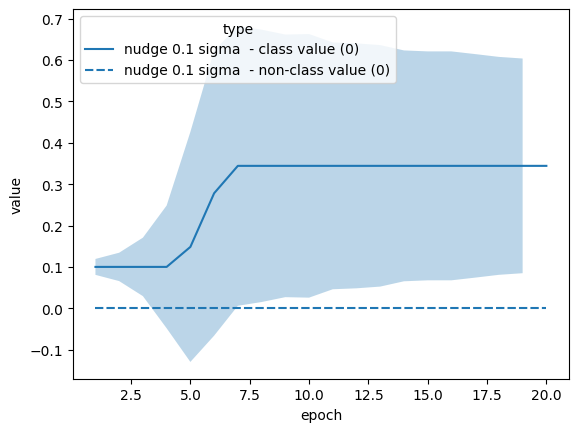
\includegraphics[width=0.5\linewidth]{graphs/sigma.png}
    \caption{Class and non-class value development over 20 epochs}
    \label{fig:class_dev}
\end{figure}

In Figure~\ref{fig:class_dev} see the class value (full) and non-class value (dotted) for class 0 in the MNIST dataset over the course of training the CNN. The blue area represents $\sigma_{sum}$, or rather, the area within a distance of $\sigma_{sum}$ from the class value. 

The class and non-class values are likely initialized to around $0.1$ and $0$ respectively during pretraining. The nudge value $\epsilon = 0.1$ suggests that both were near $0$ when initially generated and then nudged apart to their positions at the beginning of the graph.

We also observe that, as described in Algorithm~\ref{alg:sigma_spacing}, when the non-class value comes within a distance of $\sigma_{sum}$ to the class value, we attempt to move the non-class value down. Since the non-class value is already at the lower bound of $0$ here, the class value is moved up by  $\sigma_{sum}$ instead.

\subsection{Performance Comparison}
To compare the performance of these approaches, we examine accuracy over training time, focusing on both final performance and convergence speed.
\begin{figure}
    \centering
    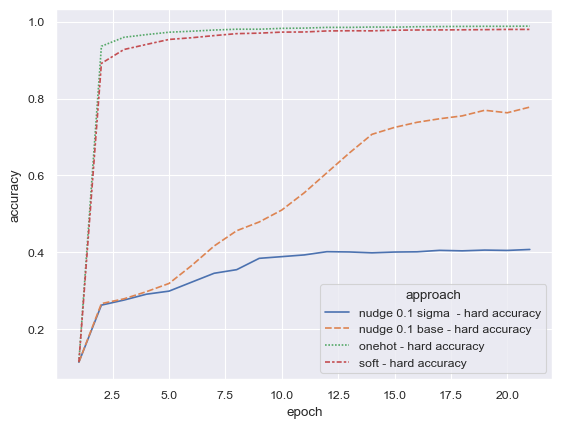
\includegraphics[width=0.6\linewidth]{graphs/acc.png}
    \caption{Accuracy Over Time}
    \label{fig:acc}
\end{figure}

As shown in Figure~\ref{fig:acc}, the one-hot and soft target approaches achieve over 90\% accuracy within the first 3 epochs. In contrast, the mean-nudge initialized model without spacing reaches just under 80\% accuracy after 20 epochs, while the variant using sigma spacing plateaus at approximately 40\% accuracy by epoch 10.
\subsection{Accuracy and Target Value Separation}
In Figure~\ref{fig:accvsep} we compare the development of accuracy with the average distance between class and non-class values in each approach.

\begin{figure}[H]
    \centering
    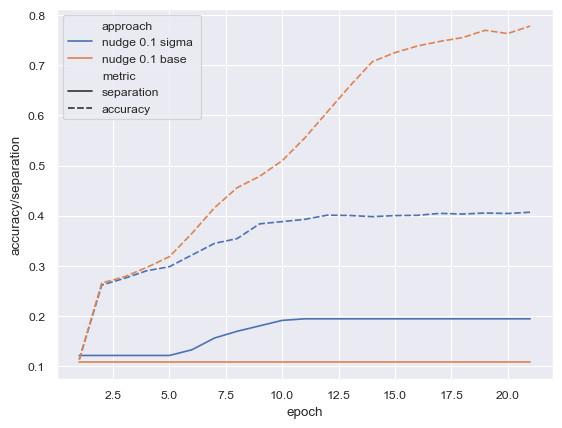
\includegraphics[width=0.6\linewidth]{graphs/accvsep.png}
    \caption{Accuracy vs. Target Value Separation}
    \label{fig:accvsep}
\end{figure}

While the sigma spacing approach gradually increases its average separation between epochs 5 and 10, the approach without sigma spacing maintains a constant separation between the class and non-class values throughout training. The sigma-spaced approach enhances its accuracy only during the initial two epochs and during the separation change, while the non-spaced approach experiences an overall increase in accuracy throughout the training process.
\subsection{Loss Development During Training}
Figure~\ref{fig:loss} shows the development of training loss over the 20 epochs for all four approaches, as well as a magnified view of just the base and sigma spacing approaches.

\begin{figure}[htbp]
\centering
\subfigure[Loss development over training epochs\label{fig:all_loss}]{%
    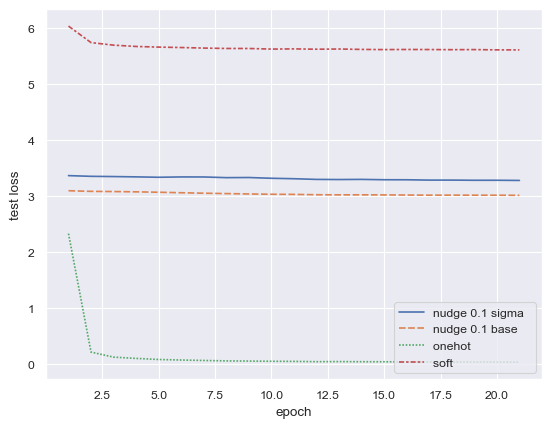
\includegraphics[width=0.48\textwidth]{graphs/loss.png}
}
\hfill
\subfigure[Loss development of base and sigma approaches\label{fig:dyn_loss}]{%
    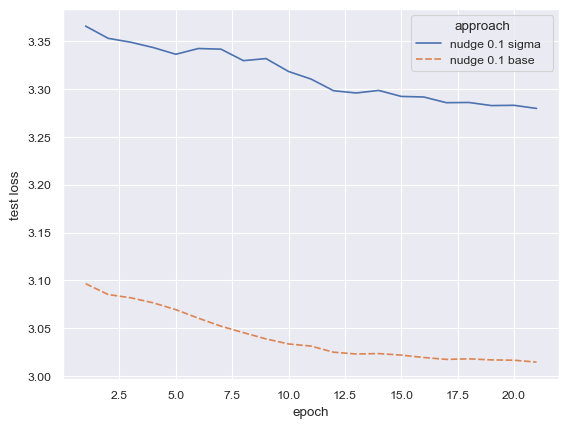
\includegraphics[width=0.48\textwidth]{graphs/lossdyn.png}
}
\caption{Training loss comparison across different target value strategies}
\label{fig:loss}
\end{figure}

The test loss of the one-hot and soft target develop in line with their accuracy, showing a steep dropoff in the first few epochs, then slowly decreasing until the end of training. The loss in our proposed approaches decreases steadily throughout the entire training, without speeding up or slowing down significantly at any point.

\subsection{Accuracy and Confidence}
In Figure~\ref{fig:accvconf}, we compare the final accuracy and confidence of the four different approaches after training for 20 epochs.
\begin{figure}[H]
    \centering
    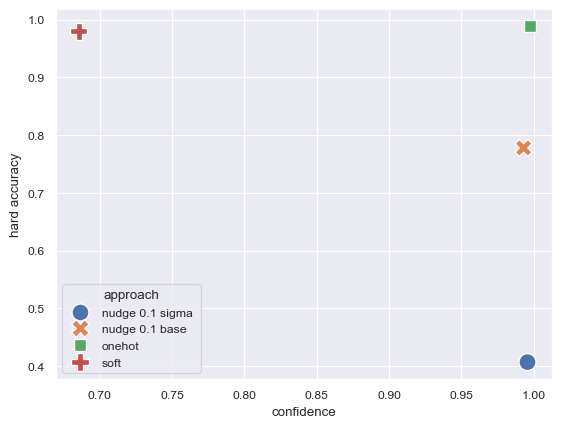
\includegraphics[width=0.5\linewidth]{graphs/accvconf.png}
    \caption{Accuracy vs. confidence}
    \label{fig:accvconf}
\end{figure}

While accuracy varies dramatically across methods (100\% for soft/one-hot targets, 80\% for mean-nudge without spacing, 40\% for sigma spacing), confidence remains consistently high ($\sim$ 100\%) for all approaches except soft targets. This creates a stark mismatch between confidence and actual performance for the mean-nudge methods.

\section{Discussion and Potential Next Steps}
The aim of this section is to analyze the results of our experiments and find potential explanations for the observed behavior, as well as to point out any meaningful correlations in our data.

\subsection{Performance Analysis: The Confidence-Accuracy Mismatch}
The core insight which can be gained from these experiments is that these novel approaches are, in their current form, not very valuable and fail to fill a useful niche. The initial goal was to achieve better training speed or reduce overfitting while maintaining useful accuracy. However, our results demonstrate that the proposed dynamic target methods deliver neither benefit: they achieve significantly lower accuracy (40-80\%) compared to traditional methods ($> 90\%$), while paradoxically maintaining high confidence ($\sim 100\%$) that undermines any potential regularization benefits (Figure~\ref{fig:accvconf}).
Where the one-hot approach delivers the best overall accuracy and training speed, the regular soft target approach exhibits similar accuracy with appropriately lower confidence, therefore acting against overfitting. Our dynamic approaches occupy the worst possible position in this trade-off space (poor accuracy combined with overconfident predictions) making them unsuitable for practical applications where either high performance or well-calibrated uncertainty is required.

\subsection{The Divergence Between Loss and Accuracy}
Where Figure~\ref{fig:dyn_loss} clearly shows the loss of our approaches decrease steadily during the entire training process, the accuracy (as seen in Figure~\ref{fig:acc}), especially of the sigma spacing approach, does not mirror this trend as might be expected. While the decreasing loss does indicate that the network is learning, it appears that the sigma spacing inhibits the translation of this learning into improved classification accuracy. A potential explanation may be that, while the predictions do overall become more similar to the correct targets, the frequent movement of the class and non-class values prevents this increase in similarity from actually resulting in the closest target vector being the one from the correct class.

While this "moving target" explanation could potentially contribute to the issue, the target values do eventually stabilize around epoch 10 (Figure~\ref{fig:accvsep}). This indicates that there exists some more profound issue with (this interpretation of) the sigma spacing approach, which drives class and non-class values into positions which are fundamentally unsuitable for effective classification.

\subsection{Target Value Dynamics and Their Impact}
While the sigma spacing approach's low accuracy and high confidence provide little hope for the methods' usefulness, the baseline median-nudge initialized approach without spacing exhibits a more salvageable accuracy / confidence ratio, potentially indicating some merit in the approach if it is developed further.

Similar techniques exist, %... go on to talk about dynamically generated soft targets

\subsection{Implications for Future Work}

\section{Conclusion}

% links go here, NOT in references
\section{Links}

\begin{itemize}
\item Project Page: \url{http://student.cosy.sbg.ac.at/???}
\item PS Page:
\url{http://www.cosy.sbg.ac.at/~helmut/Teaching/PSRobotik/}

\end{itemize}

% real scientific references
\bibliography{}		% .bib files here

\end{document}